\chapter{Analýza}
\label{analysis}
Kapitola \emph{analýza} se zaměřuje zejména na rešerše v~oblasti problémové domény a ke zjištění informací potřebných k~realizaci práce. Je rozdělena celkem na tři základní části.

V~části první se zabýváme obecnou problematikou návrhu software, často používanými koncepty, aspekty, které je třeba při návrhu zohlednit a objektově orientovaným návrhem.

Druhá část se zabývá konkrétními principy objektového návrhu, konkrétně principy \emph{low coupling}, \emph{high cohesion} a \emph{Law of Demeter}. Kromě rešerše týkající se těchto principů jsou zde demonstrovány jednoduché ukázky jejich porušení.

Poslední část se zabývá analýzou Java projektů, které budou vstupem pro validaci a analýzu. Je zde rozebráno, z~jakých souborů se projekt realizovaný v~jazyce Java skládá a~jaká je základní struktura zdrojových \verb+*.java+ souborů. Dále pak tato část obsahuje rešerši existujících nástrojů pro předzpracování zdrojových kódů do podoby vhodné pro další práci.
\section{Problematika návrhu software}
Při návrhu software se uplatňují nejrůznější přístupy, vzory, pravidla. Cílem této sekce je podat rychlý přehled o~používaných návrhových konceptech, aspektech návrhu software a objektově orientovaném návrhu. U~některých aspektů uvažujeme možnost jejich podpory pomocí vhodného nástroje. Mnoho z~uvedených pojmů a postupů je dále použito při návrhu nástroje, jehož vytvoření je jedním z~cílů této práce.

\subsection{Koncepty používané při návrhu software}
Existující koncepty návrhu software poskytují vývojářům základ, z~něhož lze odvodit a aplikovat další sofistikované metody \cite{wiki:software_design}. Většinou se jedná o~různé pohledy na způsob dekompozice systému na části realizovatelné v~konkrétním programovacím jazyce. Postupem času se vyvinula celá množina konceptů návrhu software \cite{swengineeringconcepts}. Uveďme alespoň některé:

\paragraph{Abstrakce (Abstraction)} Abstrakce je proces nebo výsledek zobecnění a redukce informačního obsahu konceptu nebo pozorovatelného jevu. Typicky ponecháváme pouze \mbox{informaci}, která je relevantní pro konkrétní účel nebo záměr.

\paragraph{Postupné zjemňování (Refinement)} Postupné zjemňování/zpřesňování představuje proces tvorby\footnote{Tento koncept byl použit i pro tvorbu této práce. Nejprve byla provedena dekompozice tématu na základní bloky (specifikace, analýza, návrh, \ldots) a poté byly \uv{rekurzivním sestupem} realizované další sekce, podsekce a nakonec i elementární součásti práce (odstavce a věty).}. Je vytvářena hierarchie dekompozicí makroskopických příkazů funkce po krocích, dokud nejsou dosaženy elementární příkazy programovacího jazyka. V~každém kroku je dekomponována jedna nebo více instrukcí daného programu do detailnějších instrukcí. Abstrakce a zjemňování jsou vzájemně komplementární oblasti.

\paragraph{Modularita (Modularity)} Systém je rozdělen do samostatných komponent nazvaných moduly (popsáno dále v~podsekci \ref{analysis-sw_design_aspects}).

\paragraph{Architektura (Software Architecture)} Tento pojem odkazuje na celkovou strukturu softwarového systému a způsoby, kterými tato struktura zajišťuje konceptuální ucelenost systému.

\paragraph{Hierarchie řízení (Control Hierarchy)} Struktura programu, která reprezentuje organizaci programových komponent a určuje hierarchii řízení. Tato struktura však nedefinuje přesné pořadí operací.

\paragraph{Strukturální dělení (Structural Partitioning)} Struktura programu může být definována jak v~horizontálním, tak vertikálním smyslu. Horizontální dělení představuje samostatné větve hierarchie modulů pro hlavní funkčnosti programu. Vertikální dělení slouží k~distribuci řízení a průběhu zpracování do jednotlivých úrovní (vysokoúrovňové rutiny a nízkoúrovňové operace).

\paragraph{Struktura dat (Data Structure)} Logická reprezentace vztahů mezi jednotlivými datovými elementy.

\paragraph{Softwarová procedura (Software Procedure)} Koncept \emph{softwarové procedury} se zaměřuje na průběh zpracovávání každého jednotlivého modulu. Na rozdíl od konceptu \emph{hierarchie řízení}, který se zabývá pouze vztahy (která komponenta je řízena kterou komponentou), se zaměřuje na návrh přesné posloupnosti kroků, které modul provádí.

\paragraph{Zapouzdření (Information Hiding)} Moduly by měly být navrhovány tak, aby informace v~nich obsažená byla nedostupná modulům, které tuto informaci nepotřebují.

\subsection{Aspekty návrhu software}
\label{analysis-sw_design_aspects}
Při návrhu software musíme vzít v~potaz velké množství aspektů \cite{wiki:software_design}. Důležitost přikládaná jednotlivým aspektům je odvozena od účelu, za nímž je software realizován. Pro některé systémy může být klíčové rozšiřitelnost, pro jiné stabilita. Mezi základní aspekty patří:

\begin{itemize}
\item \emph{kompatibilita (compatibility)},
\item \emph{rozšiřitelnost (extensibility)},
\item \emph{zotavení se z~chyb (fault-tolerance/graceful degradation)} \cite{wiki:fault-tolerance},
\item \emph{udržovatelnost (maintainability)},
\item \emph{modularita (modularity)},
\item \emph{balení (packaging)},
\item \emph{spolehlivost (reliability)},
\item \emph{znovupoužitelnost (reusability)},
\item \emph{stabilita (robustness)},
\item \emph{bezpečnost (security)},
\item \emph{použitelnost (usability)}.
\end{itemize}

Zatímco některé aspekty jsou pro tuto práci zcela nepodstatné (dobrým příkladem je \emph{balení}, které se zabývá způsobem dodávky software a podpůrných materiálů), jiné je možné podpořit pomocí vhodného nástroje. Pojďme se nyní podívat na aspekty, jejichž podpora možná je:

\paragraph{Rozšiřitelnost} Tato vlastnost znamená praktický důsledek, kdy nové funkčnosti mohou být do existujícího systému přidány bez majoritních změn ve \emph{výchozí architektuře}. Pokud by bylo možné určit pravidla, která určují základní architekturu a která je možné vynutit, bylo by možné při rozšiřování systému tato pravidla opět aplikovat, což by vedlo k~dodržení výchozí architektury.

\paragraph{Udržovatelnost} Klíčovou charakteristikou \emph{udržovatelnosti} je možnost obnovit stav systému v~rozumném čase. Příkladem mohou být aktualizace virové báze antivirových programů. Jiným příkladem může být instalace bezpečnostních aktualizací. Tuto vlastnost nelze podpořit zcela přímo, je však důsledkem ostatních vlastností (zejména \emph{rozšiřitelnost} a \emph{modularita}).

\paragraph{Modularita} \emph{Modularita} znamená, že výsledný systém sestává z~dobře definovaných a~nezávislých komponent. To vede k~lepší \emph{udržovatelnosti}. Komponenty mohou být v~takovém případě vyvíjeny a testovány izolovaně předtím než jsou integrovány do výsledného požadovaného softwarového systému. Navíc získáme dobrou možnost dělby práce v~rámci vývojového týmu pracujícího na softwarovém projektu.

\paragraph{Znovupoužitelnost} Je důležité, aby bylo možné přidávat nové vlastnosti (features) systému a provádět modifikace s~pouze omezenou nebo žádnou modifikací existujících komponent (možnost použít komponenty znovu pro jiné případy užití).

\subsection{Objektově orientovaný návrh software}
Základním vstupem pro objektově orientovaný návrh bývá (mimo jiné) \emph{konceptuální model}, případně seznam \emph{případů užití} systému. To jsou výsledky předešlé fáze analýzy. Na základě těchto informací je poté zpravidla sestavován návrh systému, který pracuje nad dříve definovanými doménovými objekty.

Klíčovými pojmy při objektově orientovaném návrhu jsou \cite{wiki:oop_design}:

\paragraph{Objekt/třída}  Objekt/třída představují těsné propojení mezi datovými strukturami a metodami/funkcemi, které nad těmito daty pracují. Každý objekt by měl sloužit samostatné funkci. Je definován svými atributy/vlastnostmi, tím co je a tím co může dělat.
\paragraph{Zapouzdření} Zapouzdření je schopnost chránit některé součásti objektu před externími entitami. To je zpravidla realizováno klíčovými slovy implementujícího programovacího jazyka, která umožňují deklarovat proměnnou jako privátní nebo chráněnou uvnitř vlastnické třídy.
\paragraph{Dědičnost} Dědičnost umožňuje nové třídě rozšířit nebo i přepsat funkcionalitu jiné třídy. Výsledná podtřída má kompletní část, která je derivována z~nadtřídy a navíc své vlastní funkce a data.
\paragraph{Rozhraní} Rozhraní představuje možnost odložení implementace metod. Je možné definovat signatury funkcí nebo metod, aniž by bylo nutné tyto metody implementovat.
\paragraph{Polymorfismus} Polymorfismus nám umožňuje nahradit objekt jeho podobjektem (instancí podtřídy). Proměnná tedy může obsahovat buď objekt nebo kterýkoliv jeho podobjekt.

Při vlastním návrhu systému se používají principy objektového návrhu (popsáno dále v~sekci \ref{analysis-oop_design_principles}) a návrhové vzory. Pro realizaci objektových systému se potom používají nejrůznější frameworky a knihovny.

\section{Analýza principů objektového návrhu}
\label{analysis-oop_design_principles}

Principy objektového návrhu reprezentují množinu pokynů, které nám pomáhají vyhnout se špatnému návrhu \cite{oop_design_principles}. Špatný návrh vykazuje zejména následující vlastnosti \cite{oop_design_principles_and_patterns}:

\begin{itemize}
\item \emph{Rigidity} -- je obtížné provést změnu v~systému protože každá změna ovlivňuje příliš mnoho dalších částí systému,
\item \emph{Fragility} -- pokud provedete změnu, mohou přestat fungovat části systému u~nichž se to nečeká,
\item \emph{Immobility} -- je obtížné znovupoužití části systému v~jiné aplikaci, protože tato část nemůže být \uv{vymotána} z~aktuální aplikace.
\end{itemize}

Autor výše zmíněného článku (\cite{oop_design_principles_and_patterns}) cituje zajímavé návrhové principy. Například \emph{Open Closed Principle}, který vyžaduje, aby se existující třídy a řešení nemodifikovaly, ale rozšiřovaly. Dalším principem je \emph{Liskov's substitution principle}, který vymezuje pravidla pro dědění tak, aby instance podtřídy mohla bezpečně vystupovat na místě své nadtřídy\footnote{Ve článku je rozebráno, jaké operace bychom neměli provádět v~děděné třídě -- je totiž možné změnit chování oddělené třídy tak, že již nemůže bezpečně vystupovat na místě svého předka.}.

Důležité je srovnání \emph{návrhových principů} s~\emph{návrhovými vzory}. Toto srovnání podává článek \cite{612257}. Zatímco aplikace návrhového vzoru představuje znovupoužití \uv{úspěšného} návrhu, princip představuje spíše obecně platné pravidlo, jehož dodržováním během návrhu bychom měli získat návrh přijatelné kvality. V~případě přesného stanovení potřebných principů by bylo možné provádět automatizovaný systematický návrh (což není, vzhledem k~mnoha aspektům popisovaným v~článku, dobře možné).

\subsection{Analyzované principy}
\label{analysis-principles_analyzed}
Na základě požadavků specifikovaných sekci \ref{requirements-principle_analysis} se budeme postupně zabývat principy \emph{low coupling}, \emph{high cohesion} a \emph{Law of Demeter}. Jedná se o~principy, které se týkají strukturální kvality kódu.

Ukázkové návrhové principy a vztahy mezi nimi jsou znázorněny na obrázku \ref{analyzed_principles}. Poznamenejme, že \emph{Law of Demeter} (dále budeme používat zkratku \emph{LoD}) je konkretizací požadavků na \emph{nízkou závislost} (\emph{low coupling}) mezi moduly.

\begin{figure}[h!]
  \centering
  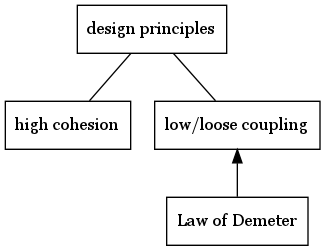
\includegraphics[width=0.5\textwidth]{./graphs/oop_design_principles.png}
  \caption{Znázornění analyzovaných návrhových principů.\label{analyzed_principles}}
\end{figure}

\subsubsection{Low coupling/dependency (nízká závislost/vazba)}
Závislost/vazba (coupling/dependency) mezi moduly softwarového projektu určuje, do jaké míry se jeden modul spoléhá na každý z~ostatních modulů \cite{wiki:coupling}. Zatímco některé moduly spolu vůbec nekomunikují (nemají žádnou závislost), jiné se spoléhají nejen na rozhraní ostatních modulů, ale mnohdy i na jejich vnitřní fungování, způsob reprezentace dat, časování atd. Důsledkem vyšší závislosti je potom nutnost rozsáhlých úprav v~mnoha modulech i při úpravě naprostých drobností v~jednom konkrétním modulu.

Proto je důležitou návrhovou zásadou snaha snížit závislost modulů na minimum. Je zřejmé, že závislost mezi moduly vždy existuje (jinak by neměl modulární návrh smysl). Proto nelze striktně říci, do jaké míry smí/nesmí být moduly na sobě závislé.

V~\cite{wiki:coupling} a \cite{STVR:STVR162} (podrobnější a formálnější definice) je podáván přehled úrovní závislosti jednoho modulu na druhém. Následující zjednodušený seznam úrovní závislostí je seřazen od nejvyšší formy závislosti po nejnižší:

\paragraph{Content coupling (nejvyšší forma závislosti)} Jeden modul modifikuje jiný modul nebo se spoléhá na vnitřní fungování jiného modulu (např. přístup k~lokálním datům jiného modulu). V~důsledku platí, že změní-li se způsob, kterým tento druhý modul produkuje data (umístění, typ, časování), povede to zcela jistě ke změnám v~závislém modulu.

\paragraph{Common coupling} Dva moduly sdílí stejná globální data (např. globální proměnnou), změna sdíleného globálního zdroje implikuje změny všech modulů, které je používají.

\paragraph{External coupling} Dva moduly sdílí externě definovaný (standardizovaný) datový formát, komunikační protokol nebo rozhraní zařízení.

\paragraph{Control coupling} Jeden modul kontroluje tok druhého tím, že mu posílá informaci o~tom, co má konat (např. předání \uv{to-do} příznaku).

\paragraph{Stamp data coupling} Jeden modul předává druhému modulu složenou datovou strukturu jako parametr. Ten ji používá pouze pro výpočty (nikoliv pro rozhodování řízení toku programu).

\paragraph{Scalar data coupling} Moduly sdílí data pomocí parametrů. Každý parametr je elementární datový typ a jedná se o~jediná data, která jsou sdílená (např. předávání celočíselné hodnoty funkci, která spočítá jeho druhou mocninu). Modul, kterému jsou předávány parametry, jich používá pouze k~výpočtu hodnoty a nikoliv pro rozhodování řízení toku programu.

\paragraph{Message coupling (nejnižší forma závislosti)} Moduly jsou komunikují pouze pomocí posílání zpráv (message passing). Jedná se o~nejnižší úroveň závislosti. Moduly o~sobě navzájem nemusí mít žádnou znalost. Moduly nepoužívají vzájemně žádné předávání parametrů, nemají žádné sdílené reference na objekty nebo globální data.

\paragraph{Independent coupling/No coupling} Mezi moduly není žádná závislost. Moduly spolu vůbec nekomunikují a nejsou zde žádné sdílené reference na proměnné nebo reference na externí data sdílená mezi moduly.

\vspace{0.5cm}

\paragraph{Subclass coupling} Pro objektově orientovaný návrh můžeme navíc uvažovat závislost typu \emph{Subclass coupling}, která popisuje vztah mezi třídou a její rodičovskou třídou. Dětská třída má závislost na rodičovské, rodičovská však žádnou závislost vzhledem k~dětské třídě nemá.

\vspace{1.0cm}

Cílem návrhu je snižovat co nejvíce míru závislosti modulů. Protože se ale jedná o~kvantitativní záležitost, nejsme schopni určit zcela přesná pravidla, která musí platit nebo která lze vynutit. U~některých typů programů může být akceptovatelný i \emph{content coupling} z~výkonnostních důvodů\footnote{Nízká vazba implikuje téměř vždy snížení výkonu z~důvodu nutnosti dalších mechanismů, které zprostředkovávají komunikaci mezi moduly (např. \emph{message passing} mechanismus).}, naopak u~jiných systémů může být nízká vazba (\emph{message coupling}) dána již návrhem (např. CORBA, web services, atd.).

\subsubsection{High cohesion (vysoká koheze/soudržnost)}
Pojmem \emph{koheze} je označována míra, jak silně související/příbuzná je funkcionalita vyjádřená modulem programu \cite{wiki:cohesion}. Existují různé přístupy k~měření této metriky, od kvalitativních, vyjadřujících se pomocí slovních ohodnocení, po kvantitativní, vyjadřující míru soudržnosti kódu pomocí čísel.

Moduly s~vysokou kohezí jsou zpravidla preferovány, protože jejich vlastnosti implikují \uv{dobré} vlastnosti návrhu včetně stability, spolehlivosti, znovupoužitelnosti a srozumitelnosti, zatímco moduly s~nízkou kohezí je obtížné udržovat a testovat.

Ke snížení koheze dochází když:
\begin{itemize}
\item funkcionalita vyjádřená třídou, ke které přistupujeme pomocí metod, nemá mnoho společného
\item metody provádějí velké množství rozdílných aktivit často nad rozsáhlými nebo nesouvisejícími daty
\end{itemize}

Nevýhodou nízké koheze je:
\begin{itemize}
\item obtížnější porozumění modulům,
\item obtížnější údržbu systému -- logické změny v~řešené doméně ovlivňují více modulů a~také proto, že změny v~jednom modulu vyžadují změny v~modulu jiném,
\item obtížnější znovupoužití modulu -- většina aplikací nepotřebuje náhodnou množinu operací, kterou modul poskytuje.
\end{itemize}

Kohezi můžeme uvažovat na různých úrovních. Jako úroveň můžeme zvolit např. metodu, třídu, balíček, modul nebo projekt. Program může mít vysokou kohezi na úrovni tříd (metody jsou dobře seskupené ve třídách podle funkcionality a pracují nad shodnými daty), zatímco na úrovni balíčků může vykazovat nižší kohezi (třídy v~rámci balíčku spolu logicky nesouvisí).

Problematikou soudržnosti programových modulů se zabývá článek \cite{Kang:1996:DCM:872750.873361}, který představuje dvě různé metriky používané k~jejímu měření.

Článek \cite{ISI:000079726000029} uvádí dělení koheze podle tzv. SMC\footnote{Podle původních autorů Stevens, Myers a Constantine.} Cohesion. Míra koheze je vyjádřena na základě typu asociace mezi procesními elementy (seřazeno od nejnižší úrovně koheze po nejvyšší):

\paragraph{Coincidental association} Neexistuje souvislost mezi elementy provádějícími zpracování.

\paragraph{Logical association} Oba elementy provádějící zpracování patří do stejné logické třídy příbuzných funkcí.

\paragraph{Temporal association} Každý výskyt obou elementů provádějících zpracování je v~tom samém omezeném časovém období při provádění programu.

\paragraph{Procedural association} Oba elementy provádějící zpracování jsou elementy stejné procedurální jednotky, která je iterativním nebo rozhodovacím procesem.

\paragraph{Communicational association} Oba elementy provádějící zpracování pracují nad stejnou množinou vstupních dat a/nebo produkují stejná výstupní data.

\paragraph{Sequential association} Výstupní data jednoho elementu jsou vstupními daty pro druhý element.

\paragraph{Functional association} Oba elementy jsou nezbytné pro provedení jedné funkce/operace.

\subsubsection{Law of Demeter}
Jak bylo zmíněno v~sekci \ref{analysis-principles_analyzed}, lze na LoD pohlížet jako na část principu pro zachování nízké vazby. LoD je také někdy nazýván jako princip nejmenší znalosti (Principle of Least Knowledge) \cite{wiki:lod}. Určuje, že každá jednotka by měla mít pouze omezenou znalost ostatních jednotek. Měla by komunikovat pouze s~omezeným počtem jednotek úzce souvisejících s~logikou této jednotky. Zde se nám částečně prolínají principy \emph{low coupling} a \emph{high cohesion}. Zatímco princip \emph{low coupling} požaduje, aby modul nezávisel na příliš detailních znalostech o~implementaci druhého modulu, \emph{high cohesion} vyžaduje, aby úzce souvisela logika modulu s~logikou závislých modulů (aby se nevolaly vzdálené logicky nesouvisející části kódu).

Princip \emph{Law of Demeter} je velmi dobře popsán v~\cite{35588}. Článek pojednává o~třídě jako o~\uv{dodavateli funkcionality}. LoD potom specifikuje, kteří dodavatelé funkcionality jsou pro konkrétní třídu preferovaní (tzv. \uv{preferred suppliers}). To nám vymezuje množinu tříd/objektů, na něž se smí vyskytnout reference v~rámci definované třídy. V~článku je rozebráno více forem principu, které jsou vhodné pro různé způsoby aplikace. Klasifikace těchto forem je znázorněna na obrázku \ref{demeter_law_types}.

\begin{figure}[h!]
  \centering
  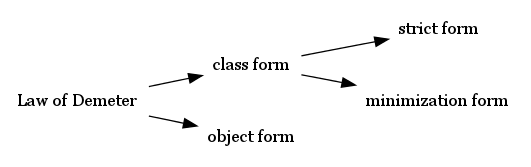
\includegraphics[width=0.7\textwidth]{./graphs/demeter_law_types.png}
  \caption{Formy návrhového principu LoD.\label{demeter_law_types}}
\end{figure}

Kromě striktní formy, která vyžaduje, aby všechny třídy dodržovaly pravidla daná principem LoD, existuje ještě minimalizační verze, která se snaží minimalizovat počet porušení pravidla pod přijatelnou mez\footnote{Například umožní porušení principu LoD v~privátním API, ale bude vyžadovat dodržení ve veřejně přístupných API.}.

Pro statickou analýzu je vhodné použití \emph{class formy} pravidla LoD. Class forma a objektová forma se lehce liší v~tom, které třídy jsou preferovanými dodavateli funkcionality. Pro praktické použití (udržovatelnost kódu, modularita, atd.) to však nemá až takový význam.

Uveďme nyní \emph{striktní třídní formu} pravidla \emph{Law of Demeter}:

\begin{designprinciple}
  Ve všech metodách M třídy C je povoleno používat pouze členy (metody a data) následujících tříd a jejich nadtříd \cite{35588}:
  \begin{itemize}
  \item C,
  \item třídy členských datových polí třídy C,
  \item třídy argumentů M,
  \item třídy, jejichž konstruktor je volán v~M,
  \item třídy globálních proměnných použitých v~M.
  \end{itemize}
\end{designprinciple}

Tento princip budeme implementovat jako ukázkové pravidlo vyvíjeného systému. Díky tomu, že je definováno na třídách a nikoliv na objektech je možné jej použít přímo nad vhodně předzpracovanými zdrojovými kódy v~programovacím jazyce Java.

\subsection{Ukázky kódu porušujícího některá z~pravidel}
Abychom demonstrovali, jak vypadá kód, který není vyhovující z~hlediska návrhu, pojďme se podívat na ukázky porušení návrhových principů. U~principu \emph{LoD} můžeme uvažovat konkrétní porušení. Pro \emph{low coupling} a \emph{high cohesion} se můžeme podívat na rozdíly mezi \emph{úrovněmi vazby} a \emph{koheze}.

\subsubsection{Porušení principu law of Demeter}
Podívejme se na nejtypičtější ukázku porušení LoD, která je uváděna v~\cite{lod:paperboy}. Zde autor demonstruje porušení principu LoD a současně modeluje reálnou situaci. Je patrné, že dodržení LoD vede k~přirozenějšímu mapování reálných objektů na objekty v~programovacím jazyce.

První částí ukázky je jednoduchá datová třída modelující zákazníka:

\lstset{
  basicstyle=\ttfamily,
  numbers=left,
  numberstyle=\tiny,
  commentstyle=\color{gray}\textit
}
\begin{lstlisting}[language=java]
public class Customer {

    private String firstName;
    private String lastName;
    private Wallet myWallet;

    public String getFirstName(){
        return firstName;
    }

    public String getLastName(){
        return lastName;
    }

    public Wallet getWallet(){
        return myWallet;
    }
}
\end{lstlisting}

Třída \verb+Wallet+ má následující definici:

\begin{lstlisting}[language=java]
public class Wallet {

    private float value;

    public float getTotalMoney() {
        return value;
    }

    public void setTotalMoney(float newValue) {
        value = newValue;
    }

    public void addMoney(float deposit) {
        value += deposit;
    }

    public void subtractMoney(float debit) {
        value -= debit;
    }
}
\end{lstlisting}

Kód pro zaplacení prodavači novin potom vypadá takto:
\begin{lstlisting}
// code from some method inside the Paperboy class
payment = 2.0; // I want my two dollars!

Wallet theWallet = myCustomer.getWallet();
if (theWallet.getTotalMoney() > payment) {
    theWallet.subtractMoney(payment);
} else {
    // come back later and get my money
}
\end{lstlisting}

Autor výše uvedené ukázky dále rozebírá, že je chybné předpokládat, že si od nás vezme pouliční prodavač novin naši peněženku, vezme si z~ní patřičný obnos a peněženku nám opět vrátí. Celá situace je vyřešena přidáním nové třídy reprezentující platbu a speciální metodou \verb+getPayment+ třídy \verb+Customer+. Zákazník se tak o~svou peněženku stará sám a prodavači pouze předá požadovaný obnos.

Ukázka nevyhoví definované class verzi principu LoD. Kód který se stará o~získání platby podle všeho dostává referenci na zákazníka. Na základě této reference získá referenci na objekt třídy \verb+Wallet+. A~právě objekt třídy \verb+Wallet+ nespadá ani do jedné z~kategorií povolených dodavatelů funkcionality (není třídou třídní proměnné, ani třídou předávanou v~parametrech, není ve třídě konstruován a není ani globální proměnnou).

\subsubsection{Ukázka kódu s~příliš vysokou úrovní závislosti}
Nejhorší variantou závislosti je závislost na konkrétním obsahu jiného modulu. Typickým příkladem může být přímý přístup k~proměnným konkrétní třídy.

\begin{lstlisting}
class A {
    public long pieceOfData;

    long getNumber() {
      return pieceOfData;
    }
}

class B {

    long computeSquare(A a) {
        return a.pieceOfData * a.pieceOfData;
    }

}
\end{lstlisting}

Tento kus kódu je špatný jednak z~hlediska zapouzdření (proměnná \verb+pieceOfData+ má být definována jako \verb+protected+ nebo \verb+private+) a dále také z~důvodu přílišné závislosti třídy B na třídě A. V~případě, že by se nám nelíbil název nebo způsob uložení proměnné \verb+pieceOfData+, změnou dojde k~nutnosti úpravy ve třídě B. Jedná se o~nejvyšší formu závislosti -- \emph{content coupling}.

Podíváme-li se na jinou úroveň závislostí, můžeme se setkat s~kódem podobným následujícímu:

\begin{lstlisting}
class A {

    int do(int what) {
        if (what == 1) {
            // do some action
            return 0;
        } else {
            // do another action
            return 1;
        }
}

class B {

    void launchAction(A a) {
        int b = a.do(1);
    }
}
\end{lstlisting}

To je typická ukázka \emph{control coupling}. Třída B využívá služeb třídy A. Metoda \verb+do+ je řízena vstupní proměnnou předávanou z~metody třídy B. To má tu nevýhodu, že v~případě změny způsobu, jakým pracuje metoda \verb+do+ (např. přidání dalšího stavu řídící proměnné) může být nutné provést reimplementaci metody třídy B, která nepočítá s~jinou návratovou hodnotou nebo jiným průběhem zpracování.

\subsubsection{Ukázka kódu s~nízkou úrovní koheze}
Nejnižší úrovní koheze je \emph{coincidental cohesion}. Typicky se jedná o~různé balíky funkcionality označované jako \verb+Utils+, \verb+Helper+ a podobně. Funkce v~takovém balíčku typicky nemají téměř žádnou příbuznost. Často se též jedná o~velké bloky funkcionality, které provádějí celou řadu nesouvisejících věcí, ale zůstávají v~jednom velkém bloku jednoduše proto, že se jich programátoři \uv{bojí dotknout}.

Příkladem úrovně \emph{logical cohesion} může být následující třída:

\begin{lstlisting}
class ErrorPublisher {

    void printErrorToTerminal(String message) {
        // implementation
    }

    void printErrorToFile(String message, File file) {
        // implementation
    }

    void logErrorToSyslog(String message) {
        // implementation
    }
}
\end{lstlisting}

Funkčnosti jsou seskupeny do jedné třídy jen z~toho důvodu, že všechny někam vypisují chybu. Každá implementace však bude zcela odlišná (metody nesdílejí žádný stav).

\section{Analýza vstupních projektů realizovaných v~jazyce Java}

V~rámci této sekce se podíváme nejprve na to, z~čeho se skládá softwarový systém realizovaný v~programovacím jazyce Java. Ve druhé části je provedena rešerše existujících nástrojů pro zpracování zdrojových kódů programovacího jazyka Java do podoby vhodné pro vygenerování potřebné vnitřní struktury, která bude předmětem validace.

\subsection{Statický model programu v~Javě}
Vstupem pro validační systém budou zdrojové kódy existujícího Java projektu ve vhodné podobě. Jedná se vlastně o~fyzický model programu. V~případě Java projektu sestává tento model z~nějaké množiny souborů, které obsahují data různých typů. První podsekce této sekce se zabývá typy souborů, které se mohou vyskytnout v~projektu, ve druhé podsekci je potom rozebírán obsah a formát souborů programovacího jazyka Java.

Zastavme se ještě nad pojmem \emph{fyzický model} programu. Tento model je zpravidla výsledkem vhodné transformace (ať už automatizované nebo ruční) nějakého předešlého modelu (většinou UML model, textová specifikace atd.). S~tímto modelem můžeme dále pracovat a provádět nad ním transformace. To je ostatně cílem různých nástrojů pro refaktoring a automatizované zvyšování kvality kódu. Konkrétně refaktoring je příkladem endogenní horizontální transformace (zdrojový i cílový meta-model je shodný a úroveň abstrakce zůstává nezměněna) \cite{Mens05ataxonomy}.

\subsubsection{Struktura softwarového projektu v~Javě}
Existuje velké množství způsobů, kterými jsou organizovány softwarové projekty. Téměř každé Java IDE má navíc svůj vlastní formát, ve kterém ukládá metadata o~projektu. Přesto všechny tyto projekty zahrnují stejnou podmnožinu konkrétních zdrojových souborů, z~nichž se skládá vlastní softwarový projekt. Podívejme se, jaké soubory můžeme nalézt v~běžném Java projektu:

\begin{itemize}
\item soubory \verb+*.java+ -- soubory se zdrojovými kódy v~jazyce Java, tyto soubory představují z~hlediska gramatiky jazyka Java kořenový element \emph{CompilationUnit} (o~něm bude dále pojednáno v~podsekci \ref{analysis-java_grammar_elements}),
\item binární součásti projektu -- soubory \verb+*.jar+ a \verb+*.class+, často se jedná o~různé knihovny, zkompilované \verb+*.java+ soubory atd.
\item build scripty a konfigurační soubory sestavovacích nástrojů (\verb+build.xml+, \verb+pom.xml+, \ldots),
\item soubory zdrojů (resources, resource bundles) -- read-only data využívaná programem (ikony, lokalizační řetězce, atd.)
\item dokumentace (\verb+javadoc+, uživatelská příručka),
\item soubory gramatik pro parsery a \emph{compiler-compiler} systémy (např. pro \verb+lex+, \verb+flex+, \verb+javacc+, \verb+antlr+),
\item šablony (typické třeba pro webové projekty, \verb+*.xhtml+ a jiné přípony),
\item konfigurační soubory (zpravidla \verb+*.xml+ soubory, často odkazují konkrétní třídy programovacího jazyka Java),
\item jiné soubory
\end{itemize}

Pro potřeby této práce jsou podstaní v~zásadě pouze soubory obsahující zdrojový kód -- soubory \verb+*.java+. Při analýze nebudeme program spouštět nebo uvažovat jeho dynamické chování (běh). Bude se jednat o~analýzu statického stavu programu (analýza struktury). Práce bude probíhat nad definicemi tříd, nikoliv nad jejich instancemi v~paměti JVM. Nejsou tedy uvažovány všechny možné běhové instance programu (všechny možné stavy objektů v~paměti virtuálního stroje).

Projekt může záviset na velkém množství dalších tříd, které nejsou součástí zdrojových kódů projektu. Tyto třídy zpracovávat nebudeme. Jedná se například o:

\begin{itemize}
\item knihovny třetích stran,
\item standardní knihovnu jazyka Java (i.e. Java 2 Platform SE 5.0 API pro Javu verze 5),
\item podprojekty a části projektu, které analyzovat nechceme, nepotřebujeme nebo z~nějakého důvodu nemůžeme (např. projekty, které nejsou pod naší kontrolou a nemůžeme u~nich návrh opravit, atd).
\end{itemize}

Některé z~těchto tříd budou povolenými závislostmi pro všechny třídy projektu (např. všechny třídy projektu mohou záviset na standardních knihovnách jazyka Java), jiné budou naopak povolené jen pro určité oblasti projektu (budeme chtít, aby rozhraní pro přístup k~databázi využívaly pouze objekty DAO vrstvy).

\subsubsection{Syntaktické elementy programovacího jazyka Java}
\label{analysis-java_grammar_elements}
Jak již bylo zmíněno v~předchozí sekci, základním kořenovým elementem gramatiky programovacího jazyka Java je \emph{CompilationUnit}. Kompletní popis všech elementů jazyka poskytuje specifikace jazyka Java \cite{Gosling:2005:JLS:1036643}.

Element \emph{CompilationUnit} dále obsahuje volitelně \emph{deklaraci balíčku}, \emph{příkazy importu} prvků z~jiných jmenných prostorů a \emph{deklarace datových typů} (obrázek \ref{toplevel_elements}). Ty jsou pro prováděnou validaci a analýzu nejdůležitější.

\begin{figure}[h!]
  \centering
  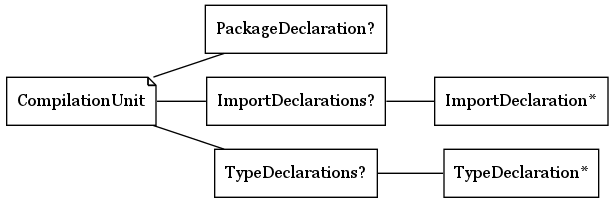
\includegraphics[width=0.85\textwidth]{./graphs/java_top_elements.png}
  \caption{Struktura základních syntaktických elementů programovacího jazyka Java.\label{toplevel_elements}}
\end{figure}

Každá deklarace datového typuje představována neterminálním symbolem \emph{TypeDeclaration} gramatiky jazyka Java. Tento neterminální symbol se dále přepisuje na symboly uvedené na obrázku \ref{type_declaration_options}. Výsledný deklarovaný datový typ může být jeden z~následujících elementů: \emph{deklarace třídy}, \emph{deklarace výčtového typu}, \emph{deklarace rozhraní} a \emph{deklarace anotace}.

\begin{figure}[h!]
  \centering
  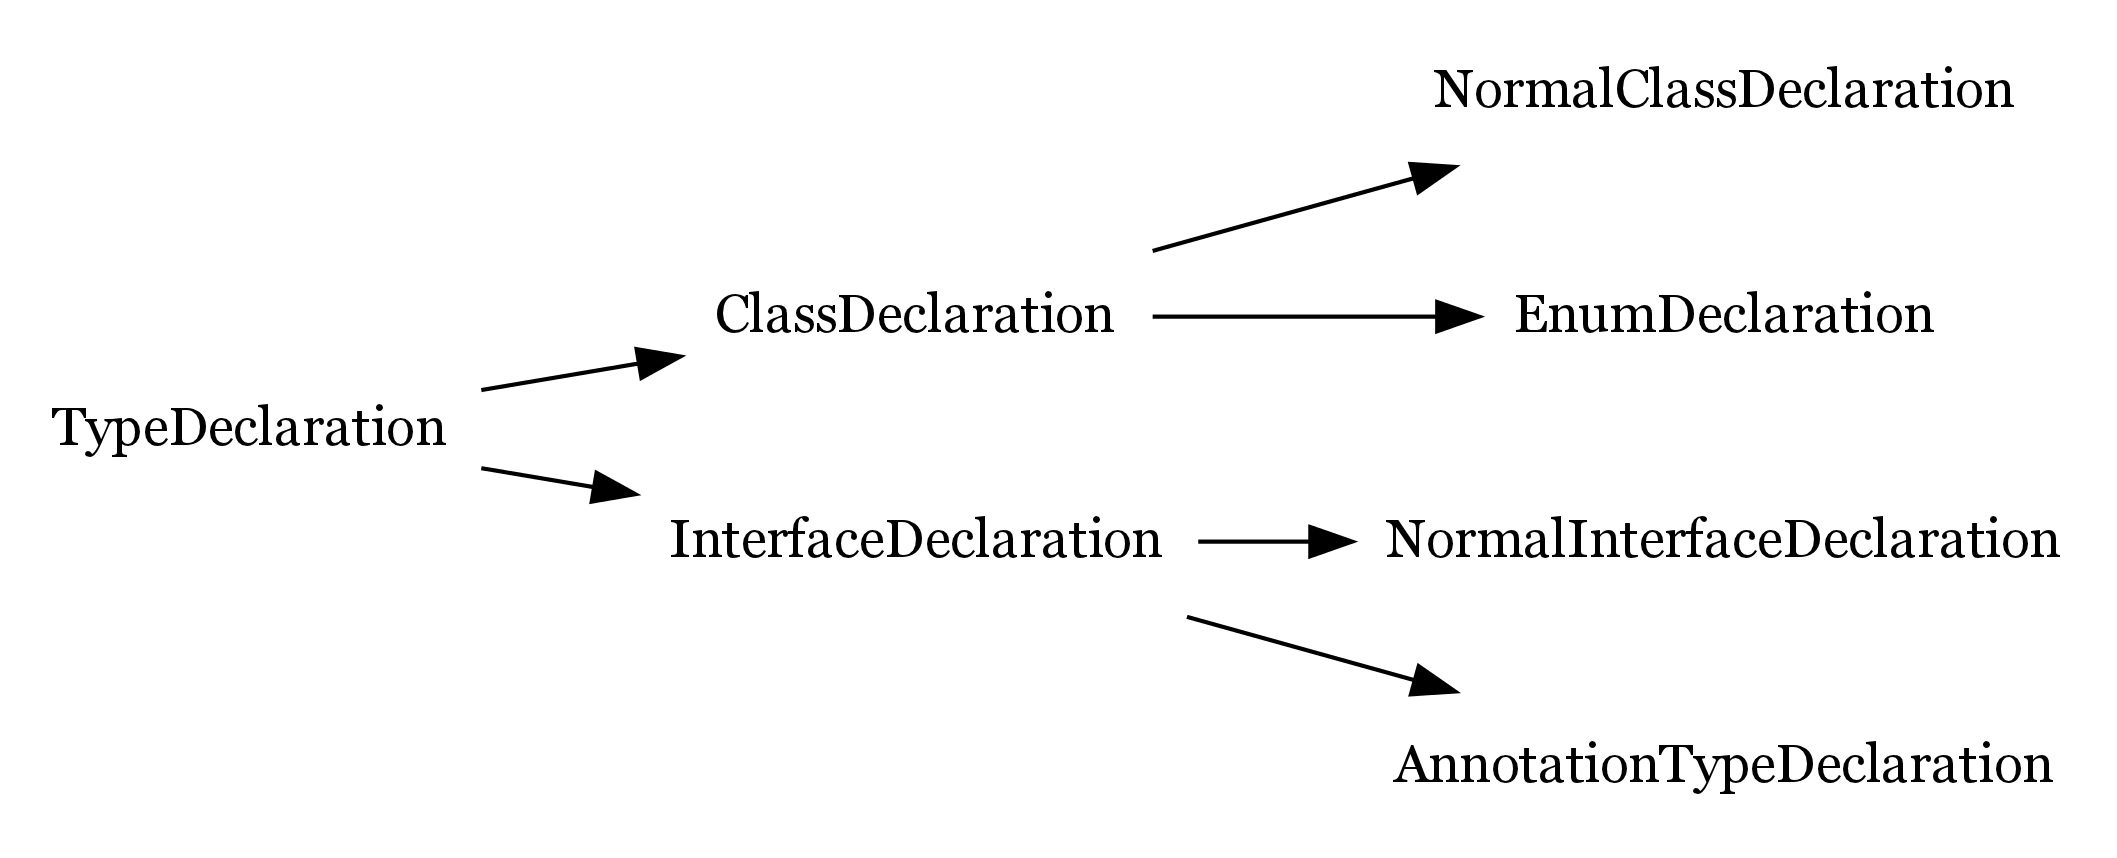
\includegraphics[width=\textwidth]{./graphs/toplevel_types.png}
  \caption{Rozklad elementu TypeDeclaration.\label{type_declaration_options}}
\end{figure}

Datové typy budou výchozími body při sestavování vnitřní reprezentace pro provádění validace a analýzy. Jejich další pod-elementy jsou tvořeny členskými proměnnými, konstruktory, metodami, abstraktními metodami (signatury metod v~rozhraních) a vnořenými datovými typy. Dále se elementy dělí až na úroveň jednotlivých příkazů, konstrukcí objektů, výrazů atd.

\subsection{Zpracovávání zdrojových kódů v~jazyce Java}
\label{analysis-java_source_processing}
Protože navrhované ověřované principy přesahují rámec jedné kompilační jednotky, je nutné provést vhodné předzpracování zdrojových kódů tak, aby bylo možné analyzovat vztahy částí kódu i mezi jednotlivými kompilačními jednotkami.

V~principu to znamená provést podobnou množinu operací, jakou provádí první kompilátor jazyka Java při kompilaci \cite{hackers_guide_to_javac}. Ten nejprve načte všechny \verb+*.java+ soubory a namapuje sekvence tokenů na uzly AST stromu. Následně vloží všechny nalezené symboly do tabulky symbolů (např. jména datových typů, proměnných atd.). Provede zpracování anotací nalezených v~kompilačních jednotkách. Ve fázi \emph{attribute} jsou provedeny operace jako rozlišení jmen, kontrola datových typů a zjednodušení konstantních výrazů. Následuje kontrola datových toků v~programu (pracuje na stromu získaném v~předchozích krocích), která má za cíl určit např. nedostupné části zdrojového kódu (po příkazu return apod.). Předposlední fáze \emph{desugar} přepíše AST a zjednoduší některé výrazy používané jako \uv{syntaktický cukr} na jednodušší výrazy. Na závěr provede kompilátor vlastní vygenerování zdrojových kódů nebo class souborů.

Pro provedení analýzy nám postačí zdrojové kódy zpracované do fáze \emph{attribute}. Jedná se o~AST s~rozlišenými jmény datových typů a proměnných. Nad těmito stromy můžeme dále pracovat.

Podívejme se nyní, jakými prostředky je možné tuto reprezentaci získat:

\subsubsection{Vlastní kód pro zpracovávání zdrojových kódů}
Samozřejmě je možné napsat pro zpracování zdrojových kódů vlastní nástroj. Zahrnovalo by to vytvoření lexikálního analyzátoru (tokenizer), syntaktického parseru (zásobníkový automat) a dalších mechanismů pro vybudování AST, rozlišení jmen, navázání proměnných a~realizaci velkého množství dalších operací.

Jedná se však o~velmi náročný a rozsáhlý systém, jehož rozsah by překračoval nejen rámec této práce, ale i možnosti jednotlivce realizovat takovou práci v~rozumném čase.

\subsubsection{Použití compiler-compiler systému}
Pro zpracování zdrojových kódů a různě formátovaného textu se často používá tzv \emph{compiler-compiler} systémů. Tyto systémy vygenerují jak lexikální analyzátor, tak syntaktický parser na základě vhodného popisu. Zpravidla se jedná o~popis ve formě BNF nebo EBNF gramatiky. Často je možné na základě specifikovaných pravidel vygenerovat i AST vhodný pro další zpracovávání.

Nejčastěji používanými nástroji jsou:

\paragraph{JavaCC} \emph{JavaCC} \cite{parsertools:javacc} je systém, pro který existuje velké množství gramatik. Mimo jiné také pro jazyk Java 1.5. Součástí distribuce tohoto nástroje je i program \emph{JJTree}, který je schopen na základě rozšířeného textového popisu gramatiky vygenerovat AST.

\paragraph{ANTLR} \emph{ANTLR} \cite{parsertools:antlr} je velmi pokročilý \emph{compiler-compiler} systém. Disponuje kompletním vývojovým prostředím, kterému nechybí vlastnosti jako zvýrazňování syntaxe, doplňování výrazů a podpora debugování (umožňuje krokovat generování syntaktického stromu).

\vspace{0.5cm}

Pro většinu \emph{compiler-compiler} nástrojů existuje velké množství vstupních gramatik pro různé jazyky. Většinou nalezneme i podporu pro jazyk Java verze 1.5\footnote{Což by pro naše účely postačovalo, protože Java 6 se od verze 5 neliší v~gramatice jazyka, ale v~poskytovaných rozhraních standardní knihovny.}.

Při použití některého z~výše uvedených nástrojů bychom se dostali na úroveň vygenerovaného AST stromu. Pro potřeby analýzy je však nutné provést ještě rozlišení jmen. To by bylo nutné provést ručně. Jedná se stále o~dost náročnou operaci.

\subsubsection{Použití vhodné knihovny nebo existujícího programu}
Další možností jsou existující knihovny a nástroje pro zpracování kódů v~jazyce Java.

Jako příklad můžeme uvést knihovnu \emph{JavaParser} \cite{parsertools:javaparser}. Jedná se o~samostatný Java projekt, který je možné zaintegrovat prostřednictvím nástroje Maven do vlastního projektu. Při bližším prozkoumání zjistíme, že se jedná vlastně o~aplikaci nástroje JavaCC (resp. JJTree) distribuovaného spolu s~gramatikou jazyka Java 1.5.

Jiným nástrojem je \emph{spoon} \cite{parsertools:spoon}. Je to volně dostupný nástroj, preprocesor kódu v~jazyce Java. Poskytuje úplný a detailní meta-model jazyka Java, kde každý element může být jak čten tak i modifikován. Dalším významným faktem je integrace nástroje do platformy Eclipse formou pluginu.

Zatímco nástroj \emph{JavaParser} neprovádí rezoluci jmen, nástroj \emph{spoon} vnitřně deleguje parsování a attribution na \verb+javac+ kompiler. Proto se v~dalších sekcích zaměříme na možnost využití některého z~nástrojů, které podobným způsobem poskytují zpracování až do požadované fáze.

\subsubsection{Použití prostředků poskytovaných platformou Java}
Jazyk Java od verze 6 poskytuje zajímavé možnosti integrace volání kompilátoru jazyka Java do kódu uživatelských programů \cite{source_code_analysis_corejavatechtips}. Jedná se o~následující aplikační rozhraní:

\begin{itemize}
\item \emph{JSR 199 -- Java Compiler API} \cite{apidoc:javacompilerapi}
  \begin{itemize}
  \item specifikuje způsoby volání překladače jazyka Java pomocí API ze zdrojového kódu programu
  \item balíček \verb+javax.tools+
  \end{itemize}
\item \emph{JSR 269 -- Pluggable Annotation Processing API}
  \begin{itemize}
  \item možnost přidání vlastního kódu pro zpracovávání anotací (a zčásti i kódu) do instance překladače
  \item balíček \verb+javax.annotation.processing+ -- zpracovávání anotací
  \item balíček \verb+javax.lang.model+ -- třídy poskytující model pro syntaktické elementy jazyka Java
  \end{itemize}
\item \emph{Compiler Tree API} \cite{parsertools:compilertreeapi}
  \begin{itemize}
  \item nestandardní rozšíření Java JDK (Sun verze)
  \item balíček \verb+com.sun.source.tree+ -- poskytuje rozhraní pro reprezentaci zdrojového kódu jako AST
  \item balíček \verb+com.sun.source.util+ -- poskytuje rozhraní pro operace nad AST
  \end{itemize}
\end{itemize}

Pomocí těchto nástrojů je možné získat poměrně snadno přístup do průběhu zpracování zdrojového kódu pomocí \verb+javac+ kompilátoru. Přístup však je na úrovni zpracovávání anotací (viz výše) a probíhá po částech (rounds). Nemáme tak k~dispozici plný AST strom, nad kterým by byla již provedena fáze \emph{attribute} \cite{hackers_guide_to_javac}.

\subsubsection{Použití prostředků současných vývojových IDE}
Většina majoritních integrovaných prostředí pro vývoj v~jazyce Java (IntelliJ Idea, Eclipse, NetBeans) provádí rozsáhlou kontrolu zdrojových kódů přímo během psaní. Programátor je upozorňován na to, že některá metoda nebo třída není definována nebo je definována s~jinými parametry. A~to v~případě, že daná třída se nachází ve zcela jiné kompilační jednotce.

To je ale přesně to, co potřebujeme pro naši práci. Proto byla provedena rešerše v~této oblasti. Byly nalezeny dva základní nástroje, které je možné použít. Jedná se o~platformu Eclipse a platformu NetBeans.

Platforma Eclipse poskytuje rozhraní, které reprezentuje Java projekt jako DOM prostřednictvím balíčku \verb+org.eclipse.jdt.core.dom+ \cite{parsertools:eclipsejdt}. Poskytovaný AST je možné procházet i~modifikovat.

Podobnou podporou poskytuje i platforma NetBeans. Ta vnitřně používá instanci \verb+javac+ kompilátoru. Přístup k~AST v~libovolné fázi (před resolvováním jmen i po této fázi) poskytuje prostřednictvím svého \emph{Java Source API} \cite{parsertools:javasourcejavadoc}.

Výhodou použití některé z~existujících platforem je navíc možnost přímé integrace do vývojového prostředí. Nevýhodou je ovšem svázanost s~tímto prostředím. To se však dá zčásti řešit vhodným návrhem jádra systému, které může být realizováno tak, aby bylo na platformě zcela nezávislé a závislost na platformě byla přidávána až integrací do konkrétního prostředí.
